\documentclass[11pt, reqno]{article}   	% use "amsart" instead of "article" for AMSLaTeX format
\usepackage{my_packages}
\usepackage{color}

\title{Foucault}
\author{Shankar Kulumani}
\date{19 September 2016}							% Activate to display a given date or no date

\begin{document}
\maketitle

\subsection*{Reference Frames}
There are two rotations of interest in this problem, namely the latitude angle and the angular rotation of the Earth. 
As a result, there are three reference frames of interest:
\begin{enumerate}
    \item Inertial \( \vecbf{e}_i\) - Inertially fixed reference frame located at the center of the Earth and aligned to the stars,
    \item Earth Fixed \( \vecbf{f}_i \) - Reference frame fixed to the surface of the Earth and rotates about \( \vecbf{e}_3 = \vecbf{f}_3 \) at a constant rate \( \Omega \),
    \item Body Frame \( \vecbf{b}_i \) - Rotation about \( \vecbf{b}_2 = \vecbf{f}_2 \) by the latitude angle \( \beta\).
\end{enumerate}
Our equations of motion are derived and defined in the body reference frame, defined by the basis vectors \( b_1, b_2, b_3\). 
Therefore, our pendulum pointing direction, defined in the body reference frame, is defined by the vector \( \vecbf{q} \in \S^2 \) which can also be expressed in terms of the basis vectors,\( \vecbf{b}_i \), as
\begin{align*}
    \vecbf{q} = q_1 \vecbf{b}_1 + q_2 \vecbf{b}_2 + q_3 \vecbf{b}_3 .
\end{align*}

We can transform a vector between each of these frames by using the rotation matrices:
\begin{align*}
    R_{EF} = 
    \begin{bmatrix} 
        \cos \Omega t & -\sin \Omega t & 0 \\
        \sin \Omega t & \cos \Omega t & 0 \\
        0 & 0 & 1
    \end{bmatrix} , \quad
    R_{FB} =
    \begin{bmatrix} 
        \cos \beta & 0 & -\sin \beta \\
        0 t & 1 & 0 \\
        \sin \beta & 0 & \cos \beta
    \end{bmatrix} ,
\end{align*}
where the notation \( R_{EF} \) represents the mapping to transform a vector in the \( \vecbf{e}_i \) frame to the \( \vecbf{f}_i \) reference frame, similarly \( R_{FB} \) represents the mapping to transform a vector in the \( \vecbf{f}_i \) frame to the \( \vecbf{b}_i \) frame.
To be consistent with the original notation we define
\begin{align*}
    R_\Omega &= R_{FB} R_{EF} , \\
    \dot{R}_\Omega &= R_\Omega S(\Omega R_{\beta}^T \vecbf{e}_3) ,
\end{align*}
where \( R_\Omega(0) = R_\beta = R_{FB} \).

Finally, we can also visualize these reference frames as shown in~\cref{fig:reference_frames}.
\Cref{fig:inertial} shows the inertial frame located at the center of the Earth.
In addition, the Earth is assumed to rotate about the \( \vecbf{e}_3 \) axis at a constant angular rate \( \Omega \).
\Cref{fig:earth_fixed} shows a reference frame that is fixed to the surface of the Earth. 
Therefore, the vectors \( \vecbf{e}_3 = \vecbf{f}_3\) are equivalent and point to the same direction in body reference frames.
Finally, \cref{fig:body} shows a pictorial representation of the pendulum in the body reference frame. 
The surface of the Earth is tangent to the \( \vecbf{b}_2, \vecbf{b}_3 \) plane, or can be approximated as the surface of the Earth assuming a flat Earth model.
The gravitational acceleration vector points toward the center of the Earth, along the vector \( -\vecbf{b}_1 \).
\begin{figure}[htbp] 
    \centering 
    \begin{subfigure}[htbp]{0.3\textwidth} 
        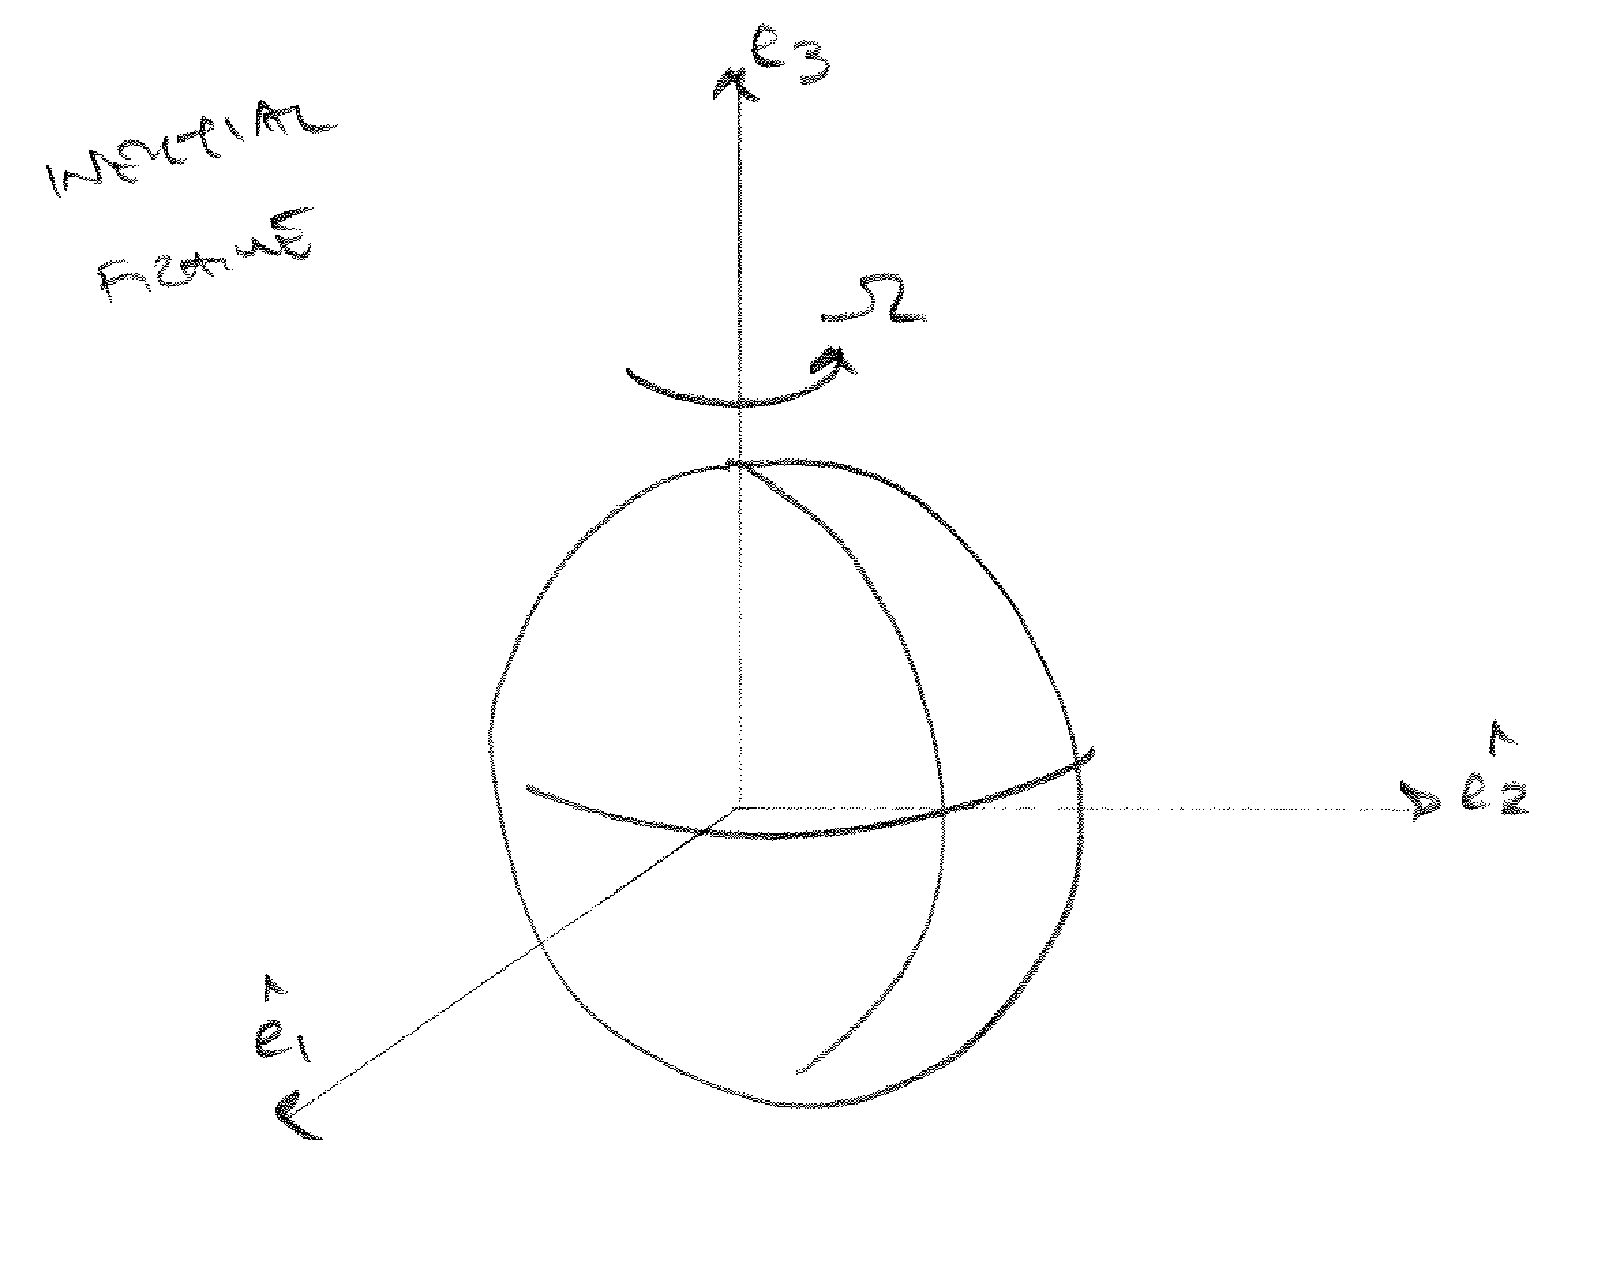
\includegraphics[width=\textwidth]{figures/inertial_frame.pdf} 
        \caption{Inertial \(\vecbf{e}_i \) frame} \label{fig:inertial} 
    \end{subfigure}~ %add desired spacing between images, e. g. ~, \quad, \qquad, \hfill etc. %(or a blank line to force the subfigure onto a new line) 
    \begin{subfigure}[htbp]{0.3\textwidth} 
        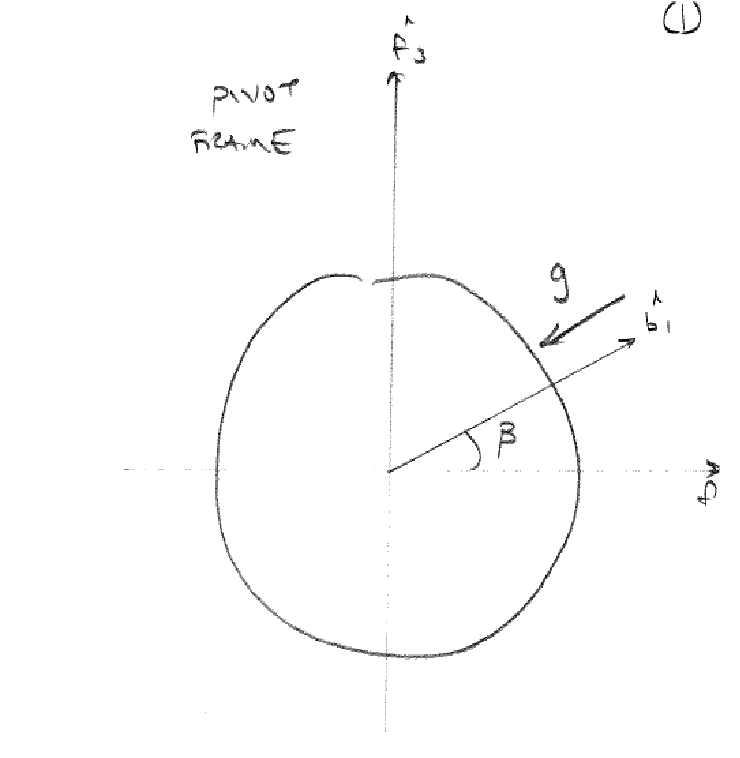
\includegraphics[width=\textwidth]{figures/earth_fixed_frame.pdf} 
        \caption{Earth Fixed \( \vecbf{f}_i \) frame} \label{fig:earth_fixed} 
    \end{subfigure}~ %add desired spacing between images, e. g. ~, \quad, \qquad, \hfill etc. %(or a blank line to force the subfigure onto a new line) 
    \begin{subfigure}[htbp]{0.3\textwidth} 
        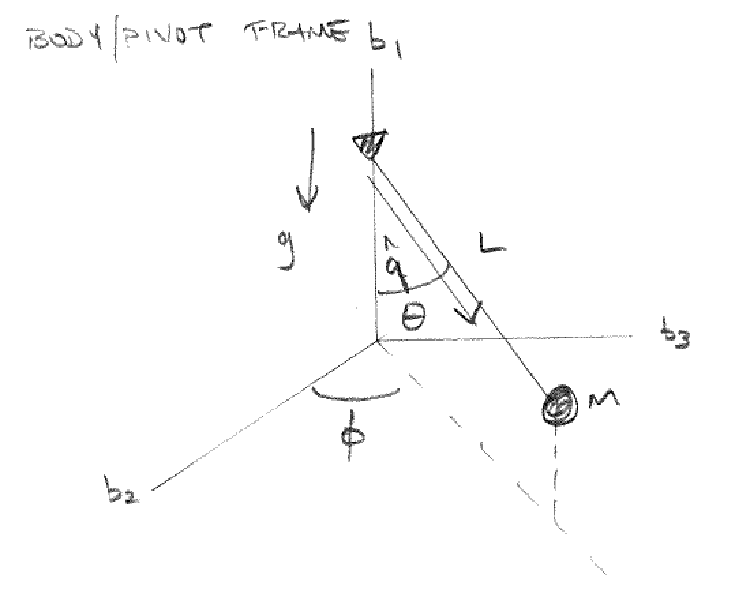
\includegraphics[width=\textwidth]{figures/body_frame.pdf} 
        \caption{Body \( \vecbf{b}_i \) frame} \label{fig:body} 
    \end{subfigure} 
    \caption{Reference Frames}
    \label{fig:reference_frames} 
\end{figure}
\subsection*{Full Nonlinear EOMS}

The total mechanical energy of the pendulum can be defined as 
\begin{align*}
    E = \frac{1}{2} m L^2 \dot{q}^T \dot{q} + m L \dot{q}^T S(\Omega R_\beta e_3) \parenth{r b_1 + L q} + \frac{1}{2}m  \Omega^2 \parenth{r b_1 + L q}^T C_\beta \parenth{r b_1 + L q} + \frac{mgr^2}{\norm{r b_1 + L q}}.
\end{align*}

The pendulum is simulated using the following parameters 
\begin{gather*}
    \Omega = \SI{7.2921158553e-5}{\radian\per\sec}, \quad L = \SI{67}{\meter}, \quad m = \SI{28}{\kilo\gram}, \\
    \quad r = \SI{6378137}{\meter}, \quad g = \SI{9.7976432222}{\meter\per\second\squared}.
\end{gather*}~
I chose two different latitude angles, \( \beta = \SI{0}{\degree} \text{ or } \beta = \SI{90}{\degree} \), to try and verify that the simulation is working correctly.
In each location the pendulum is simulated for both \( t_f = \SI{100}{s} \text{ or } \SI{3600}{s} \) to observe the energy behavior during the simulation.
The initial condition of the pendulum is defined as
\begin{align*}
    q_0 = \begin{bmatrix} -\frac{\sqrt{2}}{2} & 0 & \frac{\sqrt{2}}{2} \end{bmatrix} ,\\
    \dot{q}_0 = \begin{bmatrix}0 & 0 & 0 \end{bmatrix}.
\end{align*}
This initial state places the plane of the pendulum motion along a line of constant longitude.
In addition, this initial state should result in a complicated trajectory on the pole as well as on the equator. 

The first set of images in~\cref{fig:pole_pendulum_short} shows the trajectory and energy behavior of the pendulum at the North Pole over \SI{100}{s}.
The plane of the pendulum rotates along the \( b_1 \) axis while the energy remains well behaved with only a small variation over the time span.
\begin{figure}[htbp] 
    \centering 
    \begin{subfigure}[htbp]{0.5\textwidth} 
        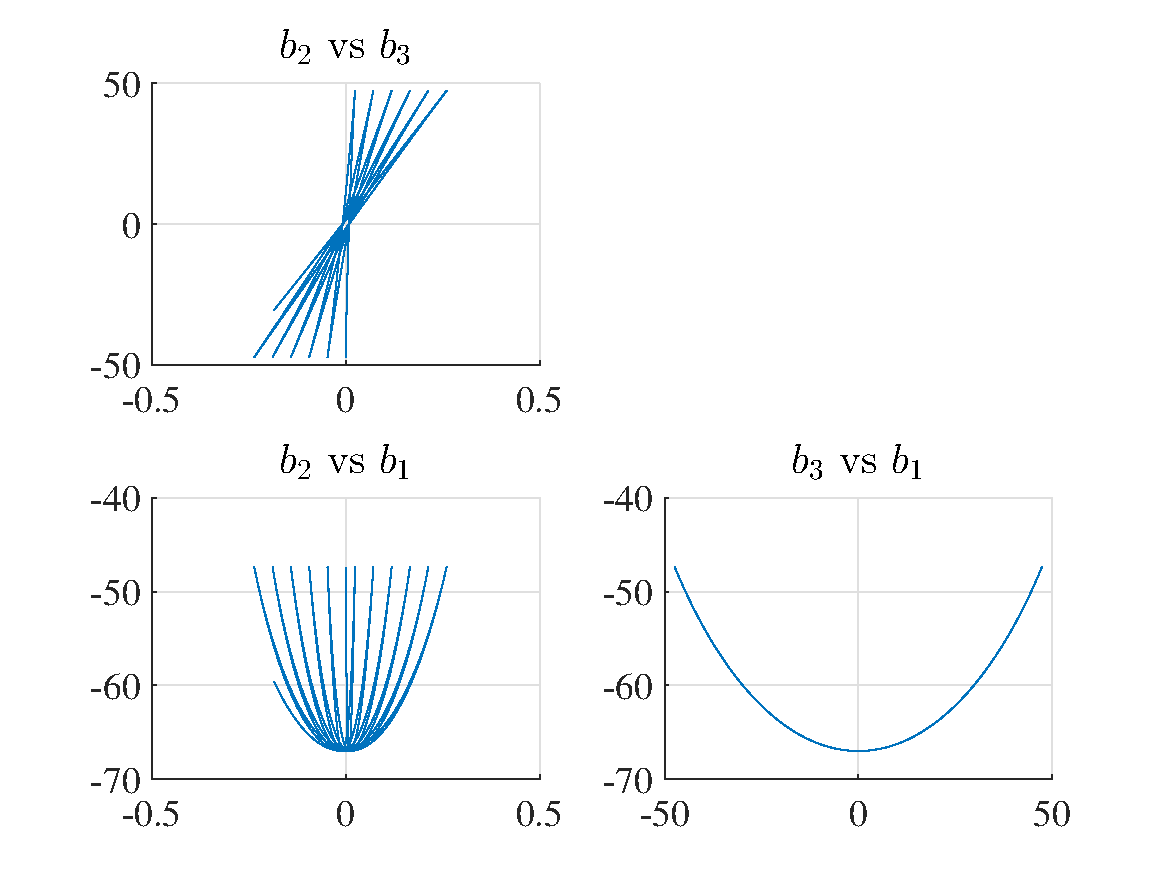
\includegraphics[width=\textwidth]{figures/pole_position_short.pdf} 
        \caption{Position } \label{fig:pole_pos_short} 
    \end{subfigure}~ %add desired spacing between images, e. g. ~, \quad, \qquad, \hfill etc. %(or a blank line to force the subfigure onto a new line) 
    \begin{subfigure}[htbp]{0.5\textwidth} 
        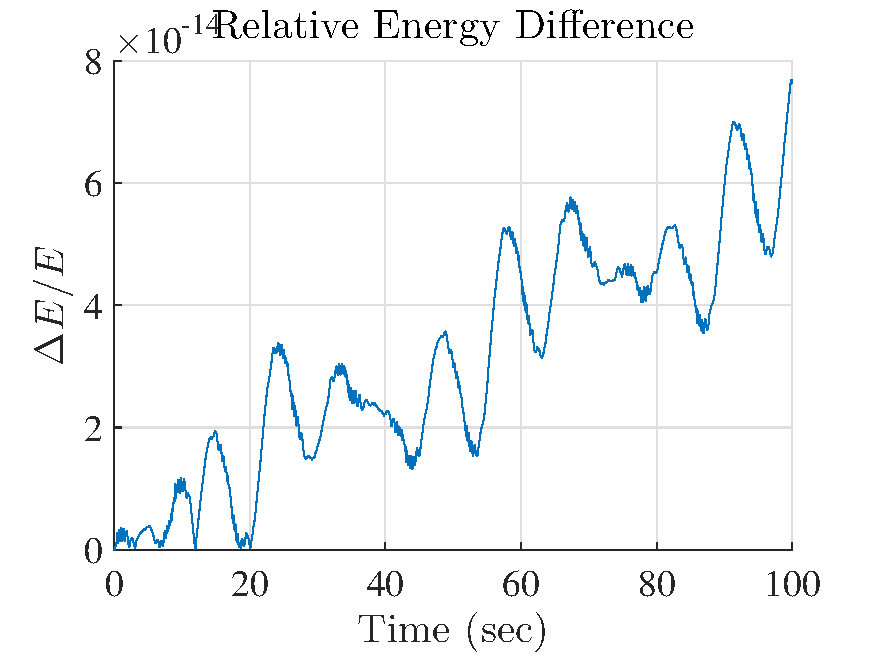
\includegraphics[width=\textwidth]{figures/pole_energy_short.pdf} 
        \caption{Energy } \label{fig:pole_energy_short} 
    \end{subfigure}
    \caption{Polar Pendulum over \SI{100}{s} and \( \beta = \SI{90}{\degree} \)}
    \label{fig:pole_pendulum_short} 
\end{figure}

Using the same initial conditions we can simulate this motion over a long time period to ensure the energy remains well-behaved.
\Cref{fig:pole_pendulum} shows the motion of the pendulum at the North Pole over \SI{3600}{s}.
These plots make the motion more difficult to observe but we can see that the plane of motion has rotated by a larger amount.
Another idea is to compute the angular rotation of the plane of the pendulum and ensure it follows the known results.
Finally, the energy seems to drift in a similar manner to what I've seen in my previous experience in the three-body problem.
The energy drift in~\cref{fig:pole_energy} is proportional to the propogation time and has some smaller local variations.
\begin{figure}[htbp] 
    \centering 
    \begin{subfigure}[htbp]{0.5\textwidth} 
        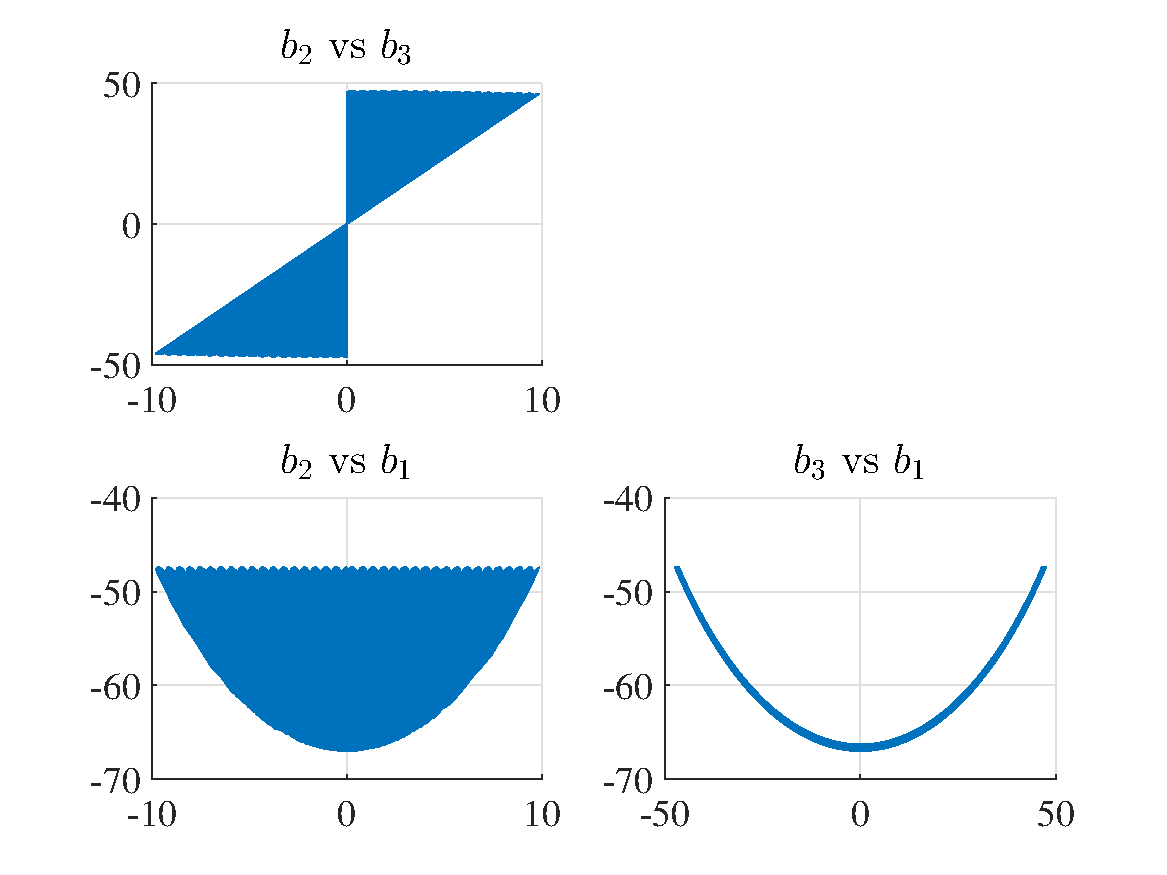
\includegraphics[width=\textwidth]{figures/pole_position.pdf} 
        \caption{Position } \label{fig:pole_pos} 
    \end{subfigure}~ %add desired spacing between images, e. g. ~, \quad, \qquad, \hfill etc. %(or a blank line to force the subfigure onto a new line) 
    \begin{subfigure}[htbp]{0.5\textwidth} 
        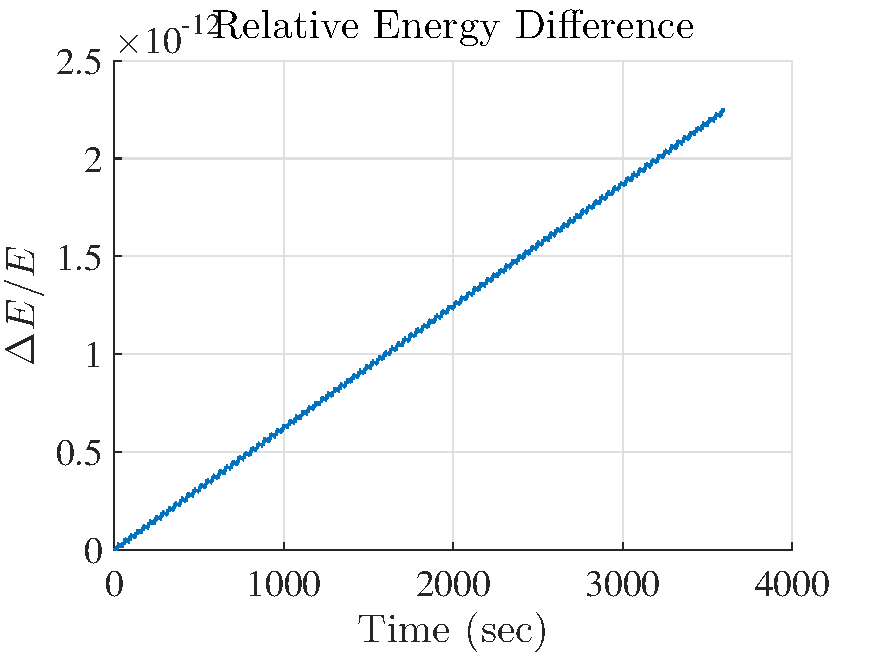
\includegraphics[width=\textwidth]{figures/pole_energy.pdf} 
        \caption{Energy } \label{fig:pole_energy}
    \end{subfigure}
    \caption{Polar Pendulum over \SI{3600}{s} and \( \beta = \SI{90}{\degree} \)}
    \label{fig:pole_pendulum} 
\end{figure}

I performed a similar simulation for both \SI{100}{s} and \SI{3600}{s} with the pendulum located on the equator, \( \beta = \SI{0}{\degree} \).
In this scenario the energy variation is much larger and no longer behaves as expected. 
The deviation of the energy is several orders of magnitude larger at the equator than at the pole. 
\begin{figure}[htbp] 
    \centering 
    \begin{subfigure}[htbp]{0.5\textwidth} 
        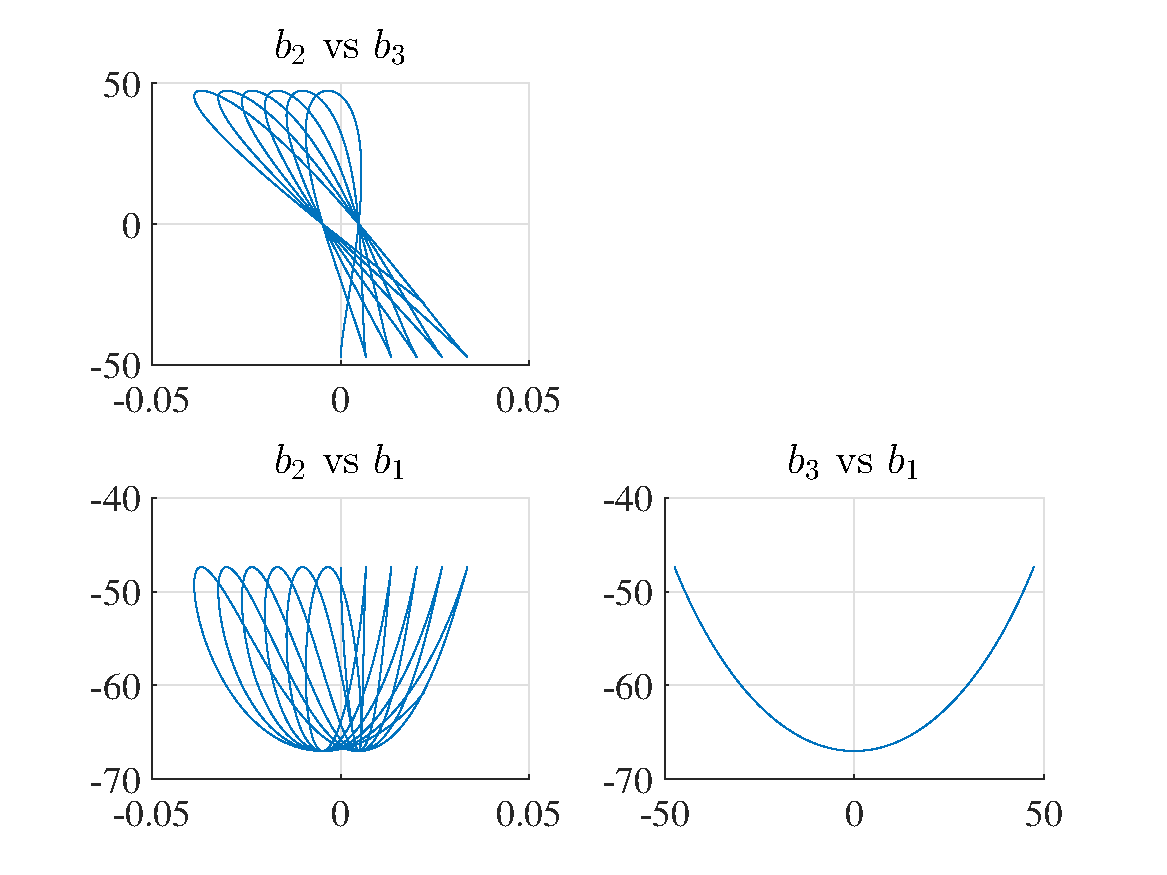
\includegraphics[width=\textwidth]{figures/eq_position_short.pdf} 
        \caption{Position } \label{fig:eq_pos_short} 
    \end{subfigure}~ %add desired spacing between images, e. g. ~, \quad, \qquad, \hfill etc. %(or a blank line to force the subfigure onto a new line) 
    \begin{subfigure}[htbp]{0.5\textwidth} 
        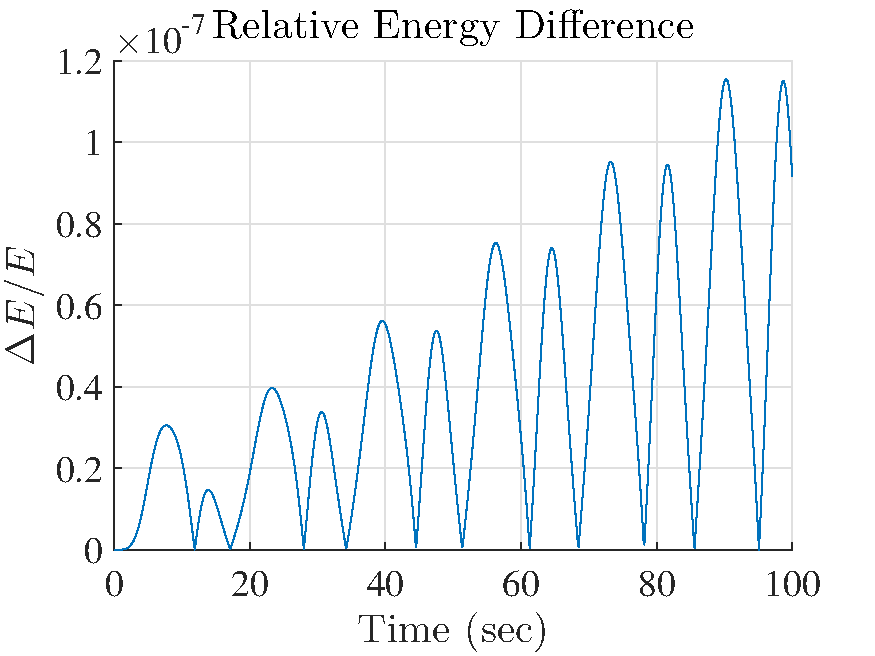
\includegraphics[width=\textwidth]{figures/eq_energy_short.pdf} 
        \caption{Energy } \label{fig:eq_energy_short} 
    \end{subfigure}
    \caption{Equatorial Pendulum over \SI{100}{s} and \( \beta = \SI{0}{\degree} \)}
    \label{fig:eq_pendulum_short} 
\end{figure}

\begin{figure}[htbp] 
    \centering 
    \begin{subfigure}[htbp]{0.5\textwidth} 
        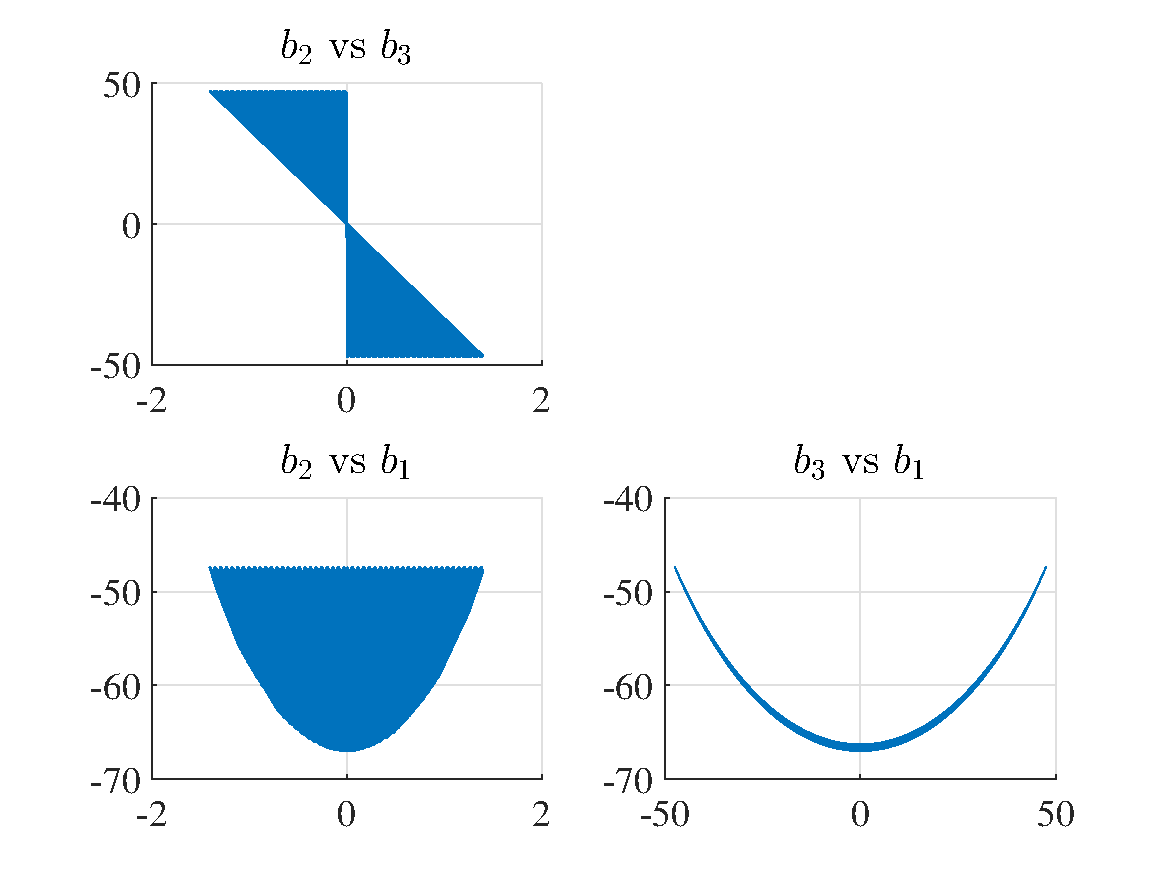
\includegraphics[width=\textwidth]{figures/eq_position.pdf} 
        \caption{Position } \label{fig:eq_pos} 
    \end{subfigure}~ %add desired spacing between images, e. g. ~, \quad, \qquad, \hfill etc. %(or a blank line to force the subfigure onto a new line) 
    \begin{subfigure}[htbp]{0.5\textwidth} 
        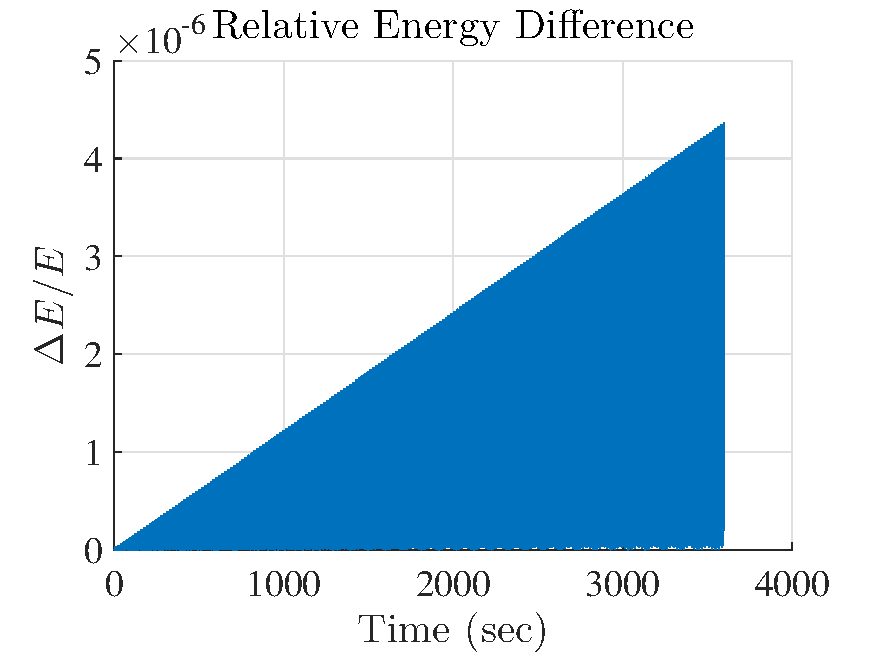
\includegraphics[width=\textwidth]{figures/eq_energy.pdf} 
        \caption{Energy } \label{fig:eq_energy}
    \end{subfigure}
    \caption{Equatorial Pendulum over \SI{3600}{s} and \( \beta = \SI{0}{\degree} \)}
    \label{fig:eq_pendulum} 
\end{figure}


\subsection*{Simplified EOMS}

The equations of motion are simplified using the assumption \( L << r \) and \(r \Omega^2 << g \) as given by Equations (3) and (4). 
The initial condition is the same as the previous example and is given by
\begin{align*}
    q_0 = \begin{bmatrix} -\frac{\sqrt{2}}{2} & 0 & \frac{\sqrt{2}}{2} \end{bmatrix} ,\\
    \dot{q}_0 = \begin{bmatrix}0 & 0 & 0 \end{bmatrix}.
\end{align*}

I performed a similar situation with the pendulum placed on the both the North Pole as well as the equator, and simulated over a short and longer time span. 

The first set of images in~\cref{fig:pole_pendulum_short_2} shows the trajectory and energy behavior of the pendulum at the North Pole over \SI{100}{s}.
There are three trajectories plotted in~\cref{fig:pole_pos_short_2} and there is very little difference between the results.
All of the trajectories are indistinguishable at this scale.
The energy behavior of the approximations are equivalent while the full-nonlinear equations are several orders of magnitude smaller.
\begin{figure}[htbp] 
    \centering 
    \begin{subfigure}[htbp]{0.5\textwidth} 
        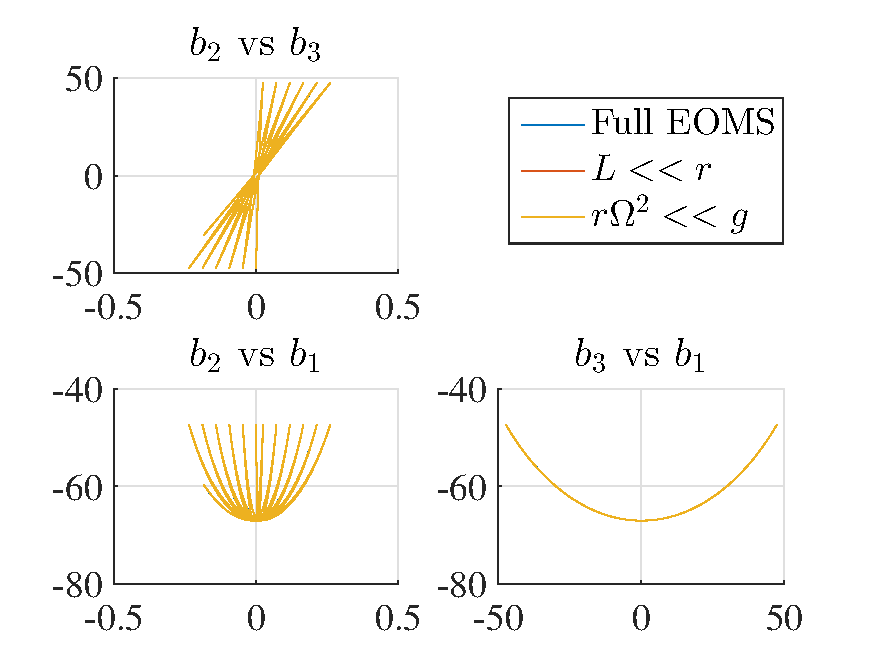
\includegraphics[width=\textwidth]{figures/pole_position_short_2.pdf} 
        \caption{Position } \label{fig:pole_pos_short_2}
    \end{subfigure}~ %add desired spacing between images, e{}. g. ~, \quad, \qquad, \hfill etc. %(or a blank line to force the subfigure onto a new line) 
    \begin{subfigure}[htbp]{0.5\textwidth} 
        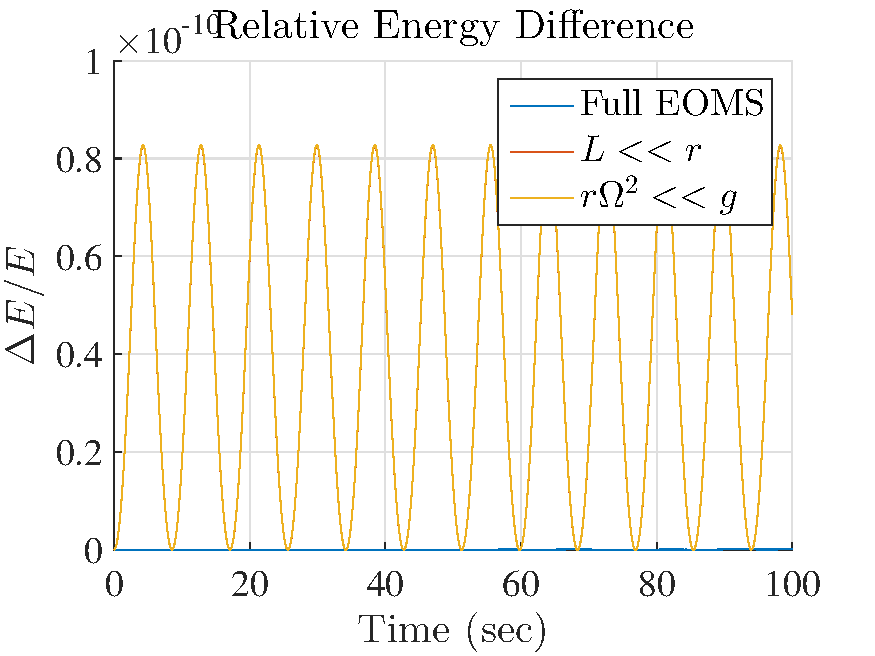
\includegraphics[width=\textwidth]{figures/pole_energy_short_2.pdf} 
        \caption{Energy } \label{fig:pole_energy_short_2} 
    \end{subfigure}
    \caption{Polar Pendulum over \SI{100}{s} and \( \beta = \SI{90}{\degree} \)}
    \label{fig:pole_pendulum_short_2} 
\end{figure}

Again, the same initial conditions are used to simulate the pendulum over a longer time span.
It's more difficult to visualize but the same behavior seen in~\cref{fig:pole_pendulum_short_2} is repeated in~\cref{fig:pole_pendulum_2}.
\begin{figure}[htbp] 
    \centering 
    \begin{subfigure}[htbp]{0.5\textwidth} 
        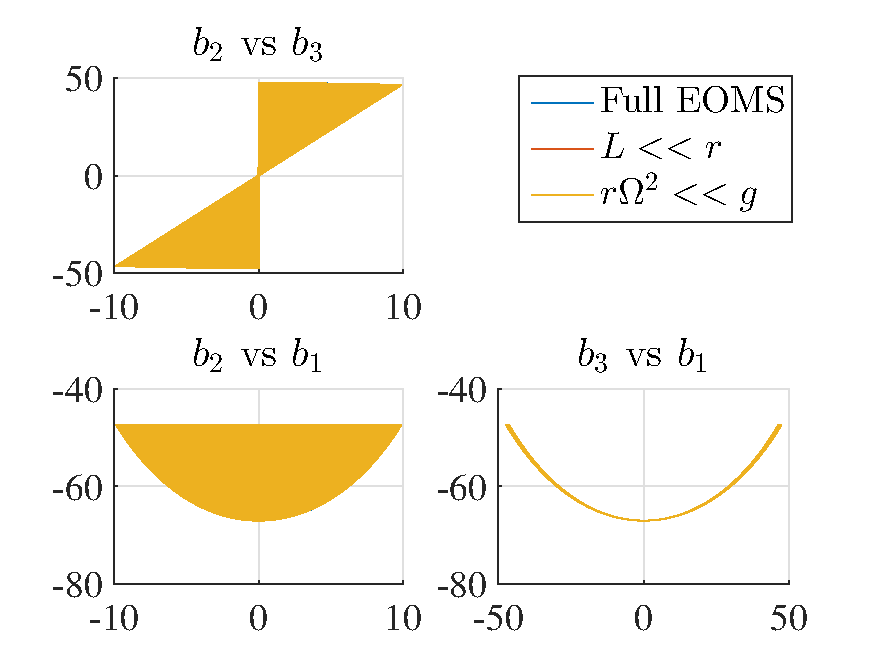
\includegraphics[width=\textwidth]{figures/pole_position_2.pdf} 
        \caption{Position } \label{fig:pole_pos_2} 
    \end{subfigure}~ %add desired spacing between images, e. g. ~, \quad, \qquad, \hfill etc. %(or a blank line to force the subfigure onto a new line) 
    \begin{subfigure}[htbp]{0.5\textwidth} 
        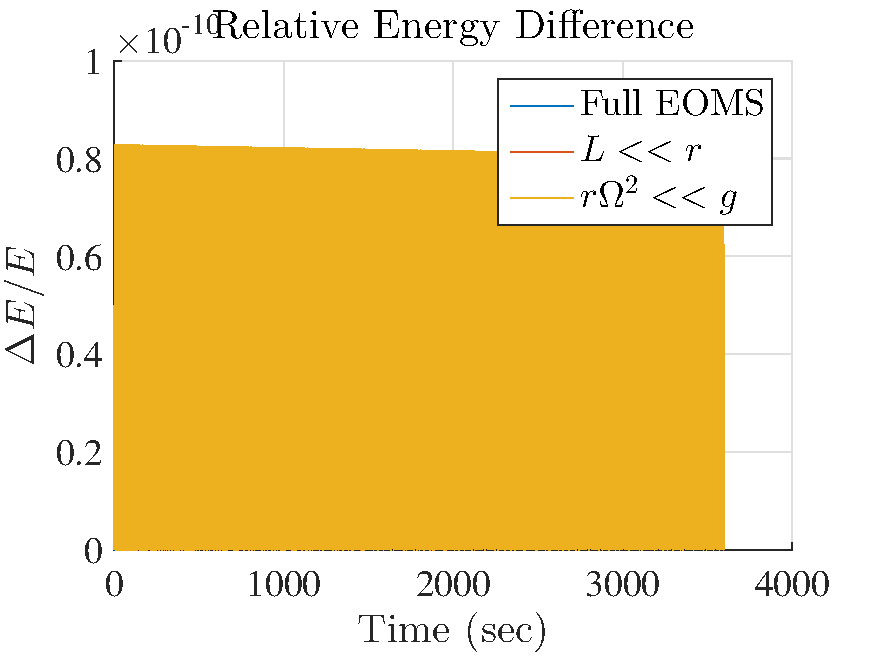
\includegraphics[width=\textwidth]{figures/pole_energy_2.pdf} 
        \caption{Energy } \label{fig:pole_energy_2}
    \end{subfigure}
    \caption{Polar Pendulum over \SI{3600}{s} and \( \beta = \SI{90}{\degree} \)}
    \label{fig:pole_pendulum_2} 
\end{figure}

I also simulated the pendulum on the equator in~\cref{fig:eq_pendulum_short_2,fig:eq_pendulum_2}.
In this case the energy behavior of the full nonlinear equations and the \( L << r\) closely match while the \( r \Omega^2 << g\) approximation is much smaller.
\begin{figure}[htbp] 
    \centering 
    \begin{subfigure}[htbp]{0.5\textwidth} 
        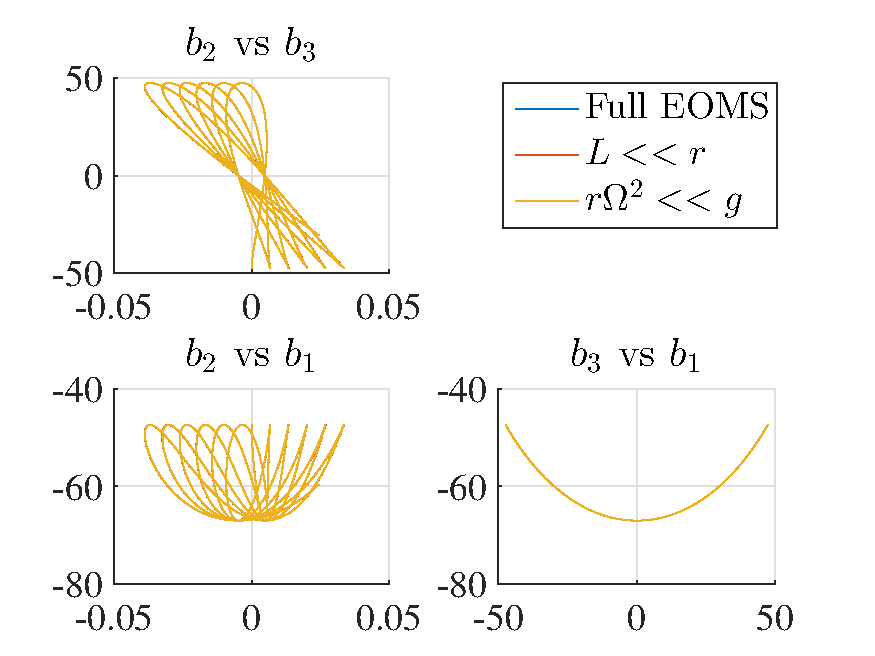
\includegraphics[width=\textwidth]{figures/eq_position_short_2.pdf} 
        \caption{Position } \label{fig:eq_pos_short_2} 
    \end{subfigure}~ %add desired spacing between images, e. g. ~, \quad, \qquad, \hfill etc. %(or a blank line to force the subfigure onto a new line) 
    \begin{subfigure}[htbp]{0.5\textwidth} 
        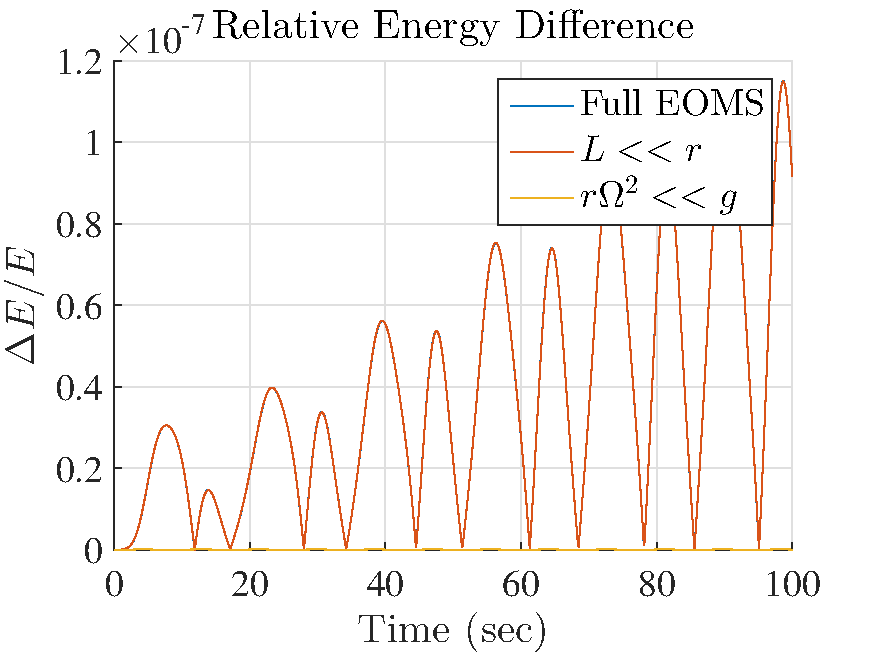
\includegraphics[width=\textwidth]{figures/eq_energy_short_2.pdf} 
        \caption{Energy } \label{fig:eq_energy_short_2} 
    \end{subfigure}
    \caption{Equatorial Pendulum over \SI{100}{s} and \( \beta = \SI{0}{\degree} \)}
    \label{fig:eq_pendulum_short_2} 
\end{figure}{}

\begin{figure}[htbp] 
    \centering 
    \begin{subfigure}[htbp]{0.5\textwidth} 
        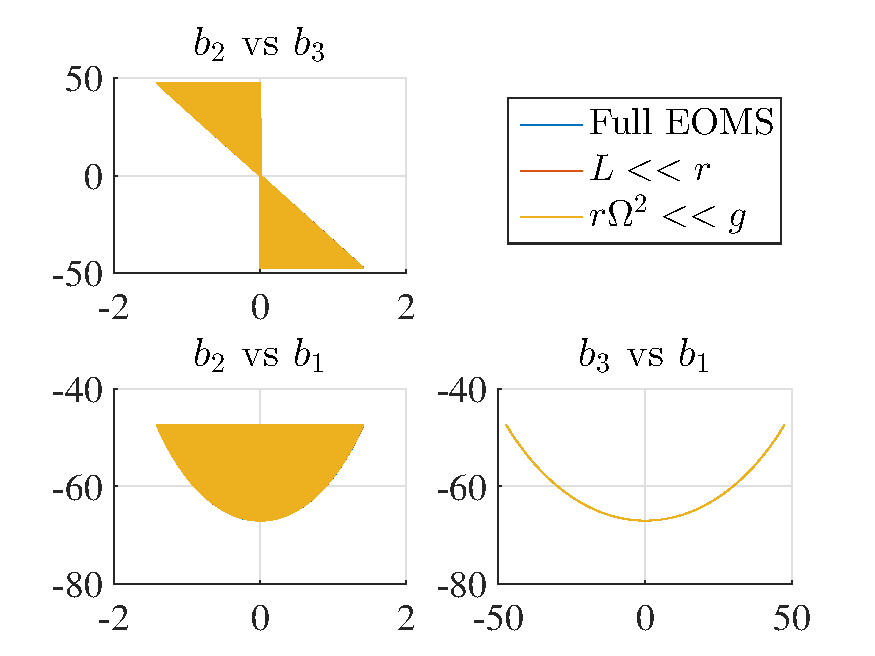
\includegraphics[width=\textwidth]{figures/eq_position_2.pdf} 
        \caption{Position } \label{fig:eq_pos_2} 
    \end{subfigure}~ %add desired spacing between images, e. g. ~, \quad, \qquad, \hfill etc. %(or a blank line to force the subfigure onto a new line) 
    \begin{subfigure}[htbp]{0.5\textwidth} 
        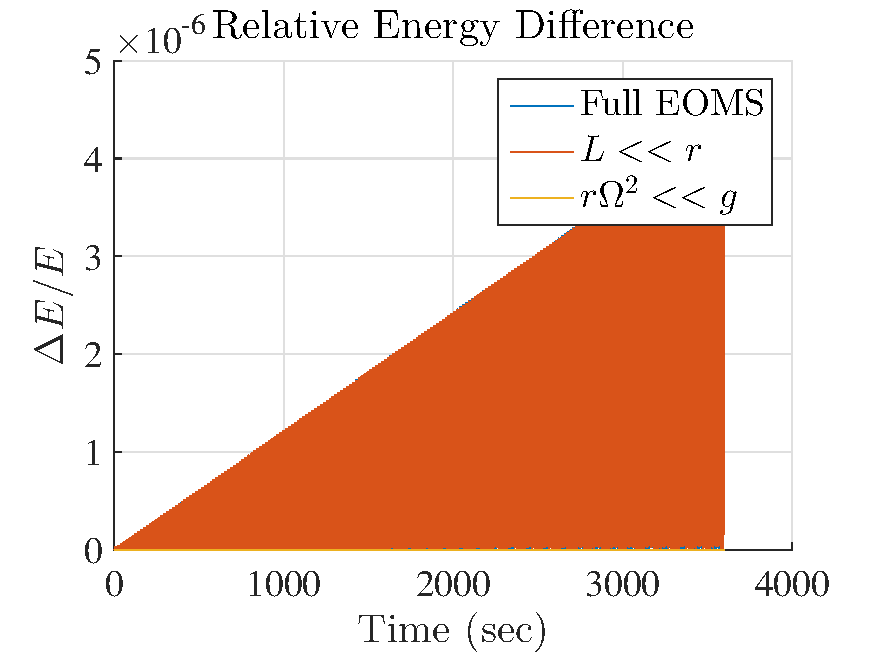
\includegraphics[width=\textwidth]{figures/eq_energy_2.pdf} 
        \caption{Energy } \label{fig:eq_energy_2}
    \end{subfigure}
    \caption{Equatorial Pendulum over \SI{3600}{s} and \( \beta = \SI{0}{\degree} \)}
    \label{fig:eq_pendulum_2} 
\end{figure}

% \bibliographystyle{abbrv}
% %\bibliography{../../../../docs/technical_papers/bibtex/library}
% \bibliography{library}
\end{document}  